\section{Implementierung}
\label{sec:implementation-analysis}

Dieses Kapitel beschreibt den Implementierungsprozess von \idename{} und erläutert einige technische Entscheidungen. Der gesamte entstandene Quelltext steht unter der \texttt{GNU} Affero General Public License~(\texttt{AGPL})\footnote{\url{https://www.gnu.org/licenses/agpl-3.0.de.html}} und ist in einem öffentlichen Git-Repository einsehbar\footnote{\url{http://blattwerkzeug.de/forward/git-repository}}. In diesem Repository befinden sich ebenfalls die Beispielprojekte aus Anhang \ref{sec:project-examples} und auch der \LaTeX-Quelltext zu dieser Thesis.

Als primäres Interface für die Kompilierung wird ein \texttt{Makefile} genutzt. Dieses prüft, ob auf dem aktuellen System alle nötigen Abhängigkeiten verfügbar sind und stellt sicher, dass Übersetzungsschritte nur ausgeführt werden, wenn sie tatsächlich notwendig sind. Von den technischen Details der unterschiedlichen Programmierumgebungen aufgrund der unterschiedlichen Programmiersprachen kann so außerdem elegant abstrahiert werden: Ein Programmierer kann sich die exakten Aufrufe der unterschiedlichen Paketmanager zwar anschauen, wird im Normallfall aber nur \texttt{make install-deps} aufrufen. Die \texttt{readme.md}-Datei im Repository erläutert diese Details zur Kompilierung und Inbetriebnahme ausführlich, sie sind daher nicht Bestandteil dieser Thesis. 

\subsection{Client-Server-Architektur}
\label{sec:implementation-client-server}

Der softwaretechnische Unterbau der Entwicklungsumgebung setzt auf aktuelle Webtechnologien auf (siehe \fullref{sec:req-web-application} für die Diskussion der Begründung) und teilt sich in zwei distinkte Codebasen für Server und Client.

\begin{description}
\item[Server: Ruby mit Sinatra] \hfill\\
  Die Aufgaben des Servers sollen sich konzeptionell möglichst auf die Auslieferung und Speicherung von Daten beschränken. Die Interaktion findet dabei primär über eine \texttt{REST}-artige \texttt{JSON}-Schnittstelle statt, serverseitig gerendert werden lediglich die Projekte der Schüler.
\item[Client: Typescript mit Angular 2] \hfill\\
  Aufgrund des hohen Grades an Interaktivität bietet sich eine rein clientseitige Visualisierung an, die weitestgehend auf Roundtrips zum Server verzichtet. Außer für den Zugriff auf serverseitige Resourcen (Datenbank, gespeicherte Ressourcen, gerenderte Seiten) werden alle Operationen im Browser ausgeführt.
\end{description}

\begin{figure}[p]
  \centering 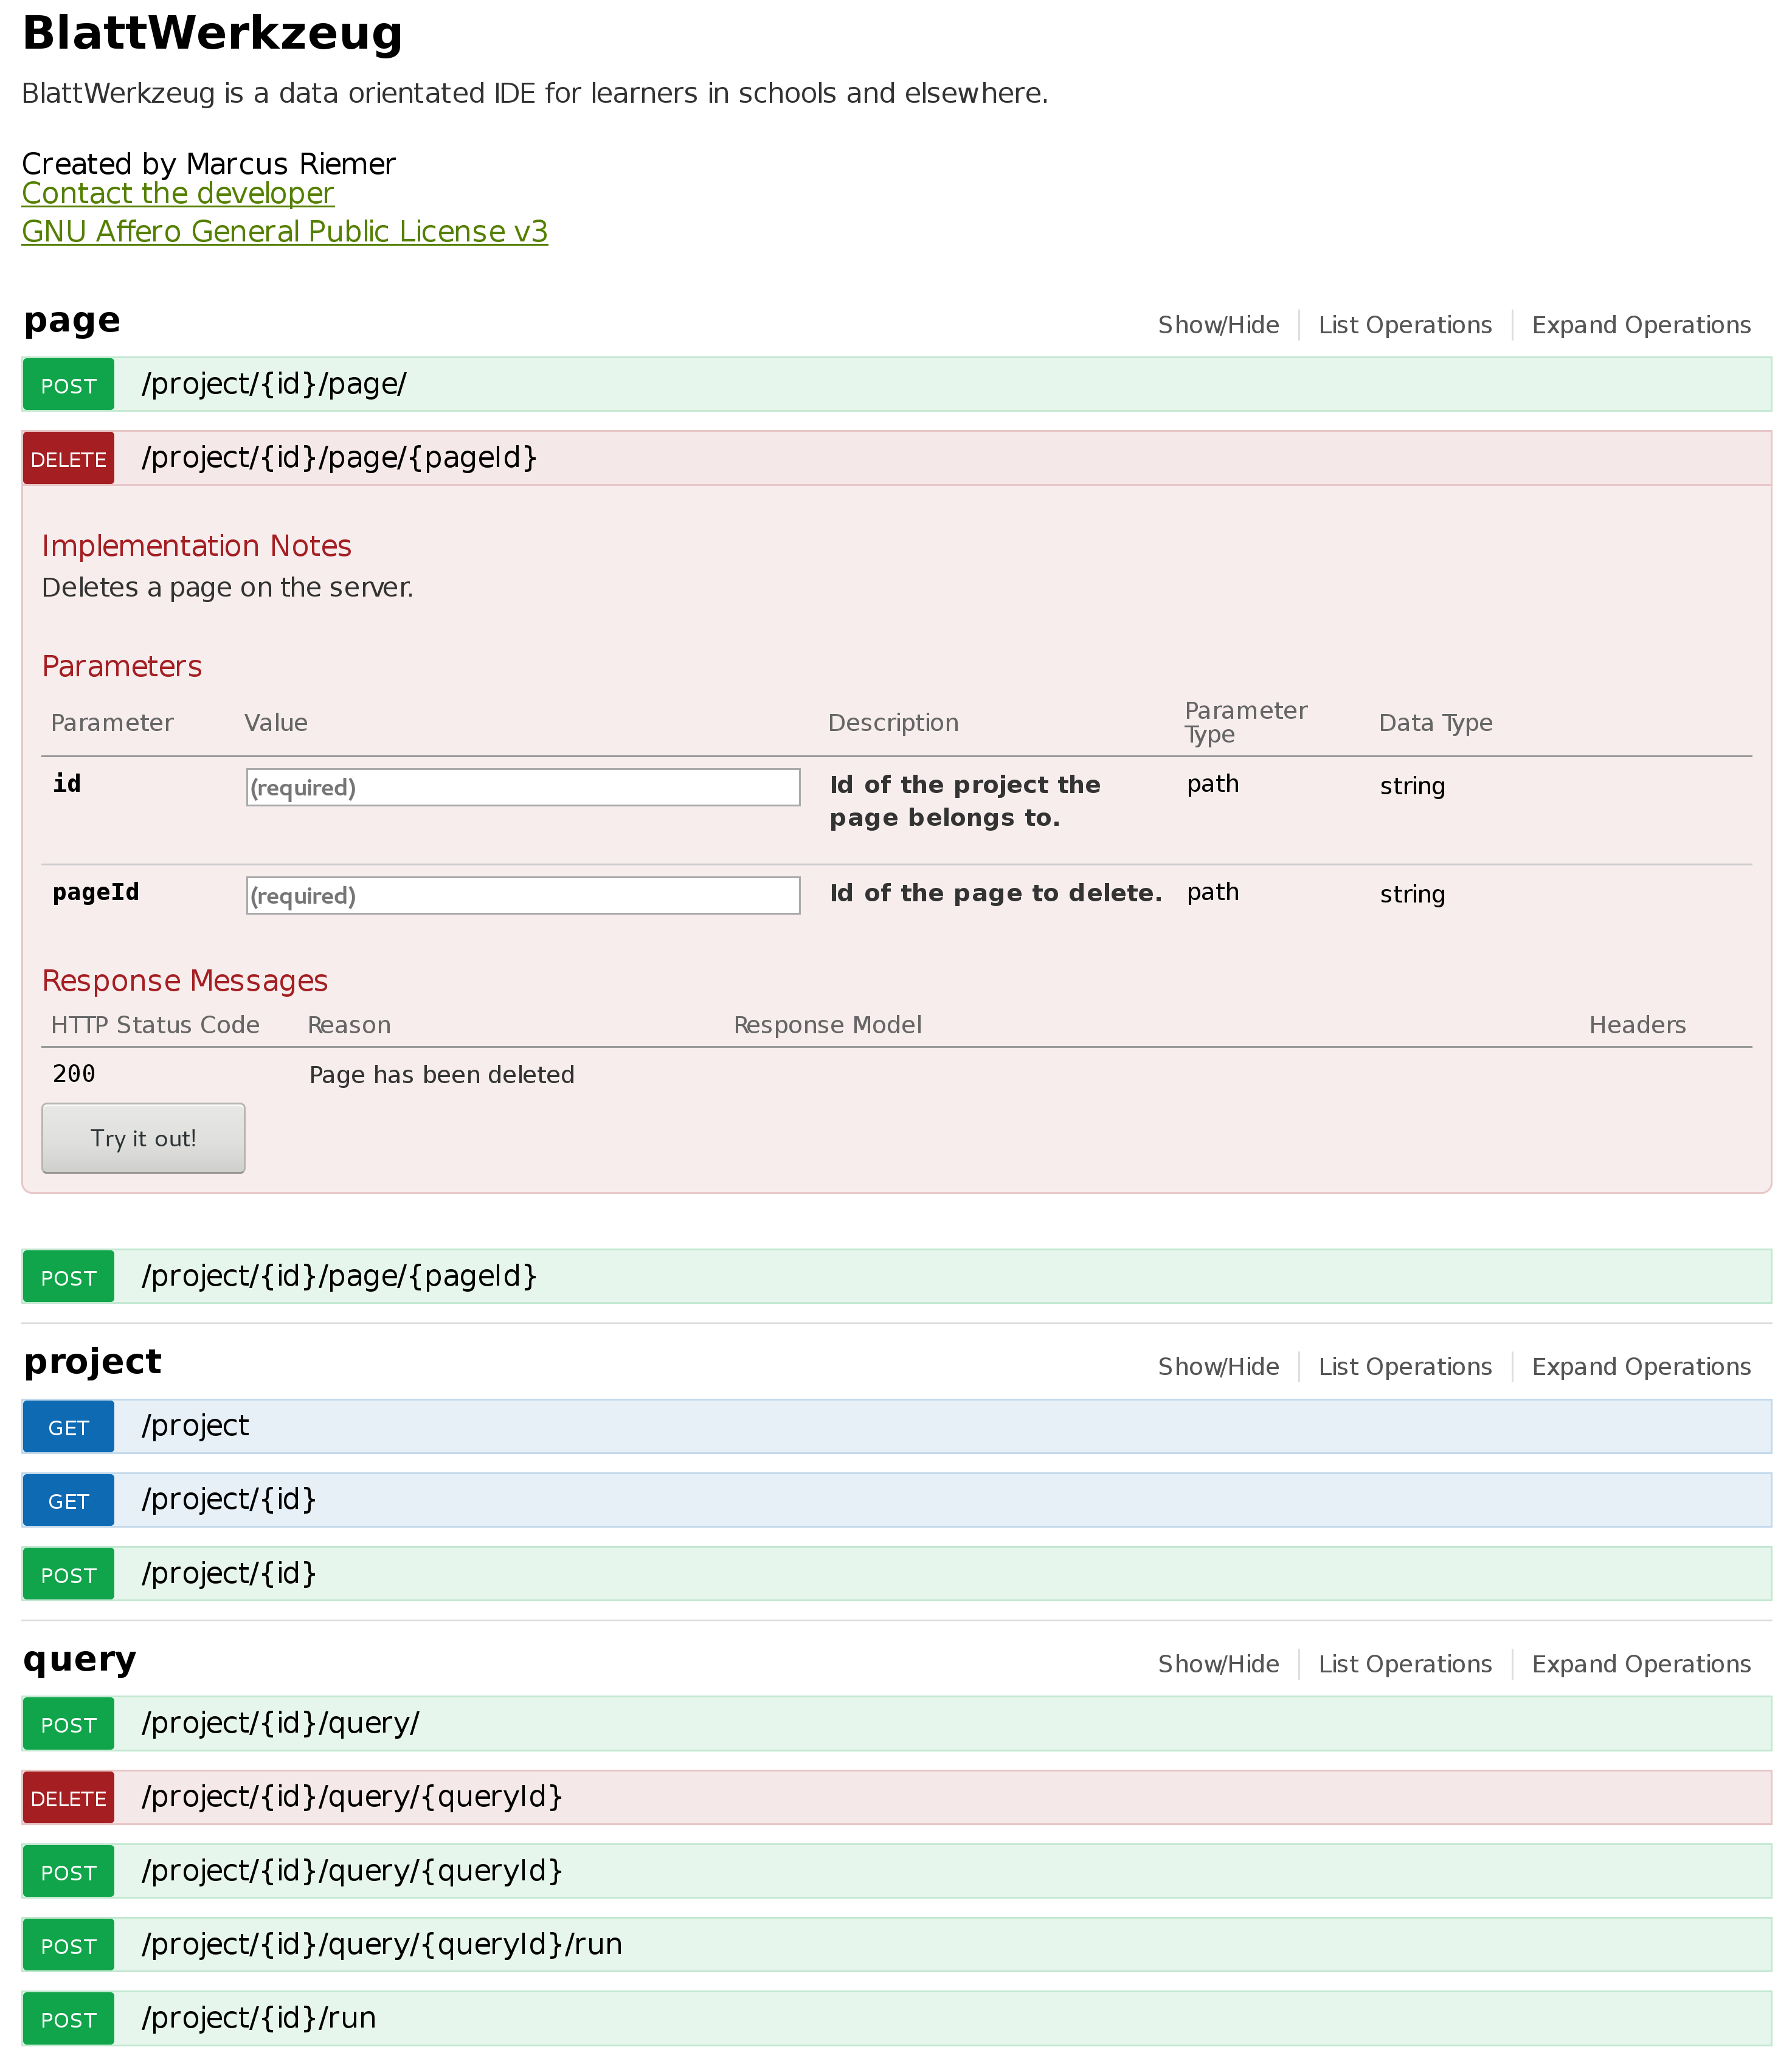
\includegraphics[width=\textwidth]{images/openapi-query-example.png}
  \caption{Generiert aus der Spezfikation: \texttt{API}-Browser für \idename{}}
  \label{fig:openapi-query-example}
\end{figure}

Um die Schnittstelle zwischen diesen beiden Komponenten so transparent wie möglich zu halten, werden diese gemäß der OpenAPI-Spezifikation\footnote{\url{https://openapis.org/}} dokumentiert. Dieses offene Format ermöglicht es, auf eine hilfreiche Auswahl an standardisierten Tools aufzubauen. Zum Beispiel können aus der Spezifikation interaktive Testumgebungen für die Server-Schnittstellen erzeugt werden, Abbildung \ref{fig:openapi-query-example} zeigt ein Beispiel dafür.

\subsection{Meilensteine}
\label{sec:implementation-roadmap}

Der Editor für Datenbankabfragen versprach im Vergleich zum Seiteneditor das einfachere Teilprojekt zu sein: Die Struktur einer Abfrage ist sehr strikt festgelegt, der Umfang lässt sich gut lokal eingrenzen. Im ersten Schritt wird allerdings nicht der komplette Editor implementiert, sondern zunächst nur das interne Datenmodell für die Abfragen in Form eines abstrakten Syntaxbaumes mitsamt den zugehörigen Tests.

Um den Umfang des Prototypen zu begrenzen, wurde die Implementierungsphase anhand der folgenden funktionalen Meilensteine geplant. Jeder Meileinstein beginnt mit einer kurzen Erläuterung und listet dann die sich daraus ergebenden funktionalen Anforderungen auf:

\begin{description}
\item[Bearbeitung von Projektdaten] \hfill \\
  Schwerpunkt dieses Meilensteins ist die Implementierung grundlegender gemeinsamer Schnittstellen. Diese müssen vom Server als \texttt{HTTP}-Endpunkte angeboten und vom Client angesprochen werden können.
  \begin{itemize}[noitemsep]
  \item Persistierung von Projekten mit Name und Beschreibung
  \item Editor für Projekteigenschaften
  \item Auflistung aller Projekte einer \idename{}-Instanz
  \end{itemize}
  
\item [Anzeige eines Datenbankschemas] \hfill \\
  Neben der funktionalen Anforderung umfasst dieser Meilenstein die Erweiterung des Clients um die typischen Bestandteile der Benutzerschnittstelle einer Entwicklungsumgebung. Serverseitig erfordert dieser Meilenstein zum ersten Mal eine Verbindung mit der Datenbank.
  \begin{itemize}[noitemsep]
  \item Editor zur Anzeige eines Datenbankschemas
  \item Seitenliste mit Übersicht über alle Bestandteile eines Projekts
  \item Toolbar mit Knöpfen, deren Verfügbarkeit vom aktuellen Editor abhängt
  \item Wechsel zwischen verschiedenen Editoren
  \end{itemize}
  
\item [Datenmodell \& Code-Generator für Abfragen] \hfill \\
  Der abstrake Syntaxbaum für Datenbankabfragen in \idename{} sowie dessen Validierung gegen ein Datenbankschema. Dieses Datenmodell soll soweit wie möglich von der Visualisierung entkoppelt werden, damit es sich möglichst einfach testen lässt.
  \begin{itemize}[noitemsep]
  \item Einfache Projektion durch Auswahl von Spalten im \texttt{SELECT}
  \item Kreuzprodukte unterschiedlicher Tabellen im \texttt{FROM}
  \item Einschränkungen der Ergebnismenge mit Ausdrücken im \texttt{WHERE}
  \item Ausdrücke mit binären Operationen zwischen Spalten, Konstanten und benutzerdefinierten Werten
  \item Validierung des Datenmodells mit im Fehlerfall aussagekräftigen Hilfen
  \end{itemize}
  
\item [Editor für Abfragen] \hfill \\
  Implementierung des Drag \& Drop-Editors für SQL-Abfragen. Wesentliche Heraus\-forderung in diesem Schritt wird die Implementierung eines möglichst allgemeingültigen Ansatzes zur Behandlung der Drag \& Drop-Vorgänge sein.
  \begin{itemize}[noitemsep]
  \item Drag \& Drop-Editor für Abfragen
  \item Ausführung von SQL-Abfragen auf dem Server
  \item Clientseitige Anzeige von serverseitigen Ergebnissen
  \end{itemize}
  
\item [Datenmodell \& Code-Generator für darstellende Webseiten] \hfill \\
  Das Datenmodell für Webseiten zur Anzeige der Ergebnisse von \texttt{SELECT}-Abfragen sowie die dazu passenden Testfälle. Auch hier gilt, dass dieses Datenmodell soweit wie möglich von der Darstellungsebene (Angular 2) losgelöst sein soll.
  \begin{itemize}[noitemsep]
  \item Layout mit Zeilen und Spalten
  \item Einfache, textbasierte Elemente wie Absätze und Überschriften
  \item Ausgabe von Abfrageergebnissen in einer Tabelle
  \item Navigation zu projekt-internen und externen Seiten
  \item Übergabe von \texttt{GET}-Parametern an Seiten
  \end{itemize}
  
\item [Rendern von darstellenden Webseiten] \hfill \\
  Um sicherzustellen, dass sich in dem Datenmodell für Seiten aus dem vorigen Meilenstein keine groben Schnitzer befinden, sollen diese nun den Endanwendern zugänglich gemacht werden.
  \begin{itemize}[noitemsep]
  \item Manuelle Erstellung einiger einfacher Testprojekte mit Testdaten
  \item Serverseitiges Rendern der verfügbaren Testprojekte
  \end{itemize}
  
\item [Editor für darstellende Webseiten] \hfill \\
  Dieser Schritt profitiert hoffentlich von den Erfahrungen mit dem Drag \& Drop-Editor für SQL. Anders als für den recht offensichtlich "`richtigen"' Ansatz des SQL-Editors hat sich im Rahmen der Analyse für diesen Meilenstein noch keine endgültig favorisierte Darstellung gefunden. Daher ist in diesem Schritt mit mehreren Iterationen bis zur "`richtigen"' Implementierung zu rechnen.
  \begin{itemize}[noitemsep]
  \item Zuordnung von \texttt{SELECT}-Abfragen zu einer Seite
  \item Drag \& Drop-Editor für Seitenelemente
  \item Integrierte Rendervorschau
  \end{itemize}
  
\item[Erweiterung der Seiten um Benutzereingaben] \hfill \\
  Bisher können mit Webseiten nur Informationen präsentiert, aber nicht verändert werden.
  \begin{itemize}[noitemsep]
  \item Einführung des \texttt{<form>}-Elementes in das Datenmodell.
  \item Eingabe von Texten mit dem \texttt{<input>}-Element.
  \item \textit{1 aus n}-Auswahl mit dem \texttt{<select>}-Element.
  \end{itemize}
  
\item [Qualitätssicherung] \hfill \\
  Zu diesem Zeitpunkt sollte ein voll funktionsfähiger Prototyp existieren, der jedoch noch einer rigorosen Qualitätskontrolle unterzogen werden muss. Bisher wurde der Prototyp ausschließlich durch Entwickler bedient, es stellt sich insbesondere die Frage, wie \idename{} auf Bedienfehler oder Inkonsistenzen reagiert.
  \begin{itemize}[noitemsep]
  \item Was passiert mit bestehenden Inhalten, wenn sich das Schema verändert?
  \item Wie sollten Seiten gerendert werden, wenn diese fehlerhaft sind?
  \end{itemize}
\end{description}

\subsection{Spontane Ergänzungen}

Sofern sich während der Entwicklung Ideen für bisher nicht bedachte Funktionalität ergaben, wurden diese in Anlehnung an den "`Minus 100 Points"'-Artikel von Eric Gunnerson geprüft\footnote{\url{https://blogs.msdn.microsoft.com/ericgu/2004/01/12/minus-100-points/}}. Die folgende Idee hat es als einzige über diese Hürde geschafft:

\begin{description}
\item[Verwendung mehrerer Datenbanken für ein einzelnes Projekt] \hfill\\
  Zu Beginn der Entwicklung galt die Prämisse "`eine Datenbank je \idename{}-Projekt"'. Diese wurde geringfügig modifiziert: "`Eine \textit{aktive} Datenbank je \idename{}-Projekt"'. Dabei standen zwei primäre Anwendungsfälle im Vordergrund: Zum Einen können auf diese Art und Weise Entwickler unterschiedliche Datenbestände mit identischen Abfragen oder Webseiten erproben. Zum Anderen lassen sich so vom Entwickler vorgenommene, serverseitig gespeicherte Backups einer Datenbank realisieren. Sofern bei einem Projekt mehrere Datenbanken zur Verfügung stehen, kann die aktive Datenbank über die Projekteinstellungen ausgewählt werden.
\end{description}

\subsection{Datenbanksystem}
\label{sec:implementation-database-system}

Die Wahl des konkreten Datenbanksystems hat einen unmittelbaren Einfluss auf nahezu alle Bereiche von \idename. Im Einzelnen handelt es sich dabei um die exakte Variante der \texttt{SQL}-Syntax, die Rahmenbedingungen für den Betrieb der Entwicklungsumgebung und auch die Fortführung der Projekte mit externen Programmen.

Die in der Praxis häufig dominierenden Entscheidungskriterien der Skalierbarkeit, die Unterstützung unterschiedlichster Zugriffsrechte und auch die allgemeine Performance spielen nur eine sehr untergeordnete Rolle. Die zu erwartenden Datenbestände sollten normalerweise im Bereich nur einiger Megabyte liegen. Die in der Praxis vermutlich einzige relevante Unterscheidung von Zugriffsrechten wäre zwischen allgemeinem lesendem und schreibendem Zugriff, nicht jedoch auf Basis einzelner Datensätze oder komplexer Benutzergruppen. Für die Wahl des Datenbanksystems werden stattdessen die folgenden Kriterien gewählt und hinsichtlich ihrer Relevanz sortiert:

\begin{description}  
\item[Kostenlose Verfügbarkeit] \hfill \\
  Der Betrieb des Datenbanksystems soll nicht mit Lizenzkosten für Schulen, Lehrkräfte, Lernende oder auch freiwillige Entwickler verbunden sein.
\item[Einfacher Betrieb] \hfill \\
  Zwar ist für den Einsatz von \idename{} aufgrund des Browsers als Client schon die Nutzung eines Servers nötig, das Datenbanksystem sollte den Betrieb aus Sicht von Administratoren der Seite dennoch nicht mehr als unbedingt notwendig verkomplizieren. Eine wesentliche Rolle spielt dabei die Plattformunabhängigkeit: Das Datenbanksystem sollte, wie auch der \idename{}-Server, auf jeder gängigen Betriebssystemfamilie (Windows, MacOS, Linux) lauffähig sein.
\item[Einfache Backups] \hfill \\
  Die gewünschte Exportfunktion für Projekte macht es nötig, den gesamten Datenbestand vergleichsweise einfach exportieren und importieren zu können. Darüber hinaus sollte es auch für Lehrkräfte möglichst einfach sein, mit allen Projekten zu einem anderen \idename{}-Server umzuziehen.
\item[Tools zur Modellierung] \hfill \\
  Da diese Arbeit sich nicht mit der Datenmodellierung befasst, muss das entsprechende Datenbankschema extern erzeugt werden. Von einer guten Unterstützung für Modellierungsvorhaben profitiert dementsprechend indirekt auch \idename.
\item[Externe Tools zur Entwicklung von SQL-Abfragen] \hfill \\
  Sobald ein Entwickler an die Grenzen des \texttt{SQL}-Editors von \idename{} stößt, soll es bei Bedarf so einfach wie möglich sein, die entsprechend komplizierten Abfragen in einem externen Editor zu schreiben und danach in Textform wieder an \idename{} zu übergeben.
\end{description}

Das Kriterium der "`kostenlosen Verfügbarkeit"' ist dankenswerterweise sehr einfach zu erfüllen: Es existiert eine Vielzahl von praktisch eingesetzten quelloffenen Datenbanksystemen. Die Kriterien "`einfacher Betrieb"' und "`einfache Backups"' teilen die denkbaren Systeme recht eindeutig in zwei Lager: Eingebette Datenbanken lassen sich sehr einfach betreiben und sichern. Das Starten eines weiteren SQL-Server-Prozesses ist bei dieser Betriebsart nicht nötig, der Im- oder Export des gesamten Datenbestandes erfordert nur die Kopie einer einzigen Datei.

Um den Betrieb folglich so einfach wie möglich zu halten, wurden für \idename{} nur eingebettete Datenbanksysteme betrachtet. Aus der Masse an verfügbaren Systemen sticht das SQLite-System jedoch sehr weit hervor: Der Quelltext ist gemeinfrei, die Anbindung an so ziemlich jede Programmiersprache ist bequem möglich und es existiert eine Fülle von verschiedensten Modellierungsprogrammen für alle Betriebssysteme. Auf eine genauere Analyse der zur Verfügung stehenden Alternativen wurde daher verzichtet.

\subsection{Tests}
\label{sec:implementation-tests}

Die Funktionalität der relativ isolierten und daher gut zu testenden internen Datenmodelle samt den darauf definierten Operationen wird über Unit-Tests sichergestellt. Diese Tests können einfach in jedem Browser ausgeführt werden und eignen sich daher auch, um im Zweifelsfall unterschiedliche Verhaltensweisen verschiedener Browser zu erfassen.

Als technisches Fundament wird für diese Testfälle auf der Jasmine-Bibliothek aufgebaut. Zu prüfende Zusicherungen werden durch Verkettung zweier Funktionen ausgedrückt: \texttt{expect().toEqual()}. Neben \texttt{toEqual()} sind natürlich auch andere Vergleiche wie \texttt{isUndefined()} möglich. Wenn innerhalb eines Testfalls auch nur eine einzige dieser Prüfungen nicht zu \texttt{true} auswertet, wird der Testfall als ingesamt fehlgeschlagen markiert. Im Falle von mehreren gescheiterten Prüfungen werden dabei alle unerwarteten Ergebnisse aufgelistet.

\lstinputlisting[
  language=javascript,
  caption=Unit-Test für eine korrekte \texttt{SELECT}-Abfrage,
  label=lst:unit-test-example,
  float=p,
  numbers=left
]{snippets/unit-test-example.ts}

\lstinputlisting[
  language=javascript,
  caption=End-to-end Test für den Speichervorgang eines Projektes,
  label=lst:e2e-test-example,
  float=p,
  numbers=left
]{snippets/e2e-test-example.ts}

Listing \ref{lst:unit-test-example} illustriert, wie die meisten Unit-Testfälle in \idename{} aufgebaut sind. Jeder Testfall beginnt mit der Definition eines Datenmodells (Zeilen 6 bis 13) und endet mit Zusicherungen, um die korrekte Serialisierung sicherzustellen (Zeilen 21 und 22). Ganz konkret existiert also in jedem Testfall eine Variable \texttt{model}, welche im Konstruktor der zu testenden Klasse zum Einsatz kommt und in nicht-mutierenden Testfällen als Ergebnis der \texttt{toModel()}-Methode reproduziert werden muss. Für Abfragen muss noch die Generierung der korrekten \texttt{SQL}-Anweisungen geprüft werden, im Beispiel geschieht dies in Zeile 20.

Die serverseitige Funktionalität wird aktuell ausschließlich über "`end-to-end"'-Tests mit einem speziell instrumentierten Browser geprüft. Für diese Tests ist ein speziell vorbereitetes Testprojekt in einem exakt definierten Zustand Teil des Repositories. Auch diese Testfälle nutzen die von Jasmine bereitgestellten Zusicherungen mit den \texttt{expect()}- und \texttt{toEqual()}-Verkettungen. Listing~\ref{lst:e2e-test-example} zeigt, wie mit einem solchen Test die Funktionaliät des Editors für Projekteinstellungen sichergestellt wird. Mittels der \texttt{browser.get()}-Funktion kann zu einer bestimmten Seite navigiert werden. Um mit den einzelnen Bedienelementen dieser Seite interagieren zu können, müssen diese anhand ihrer \texttt{ID} oder anderer eindeutiger Merkmalen zugreifbar sein (Zeilen 6, 8 und 14 des Listing~\ref{lst:e2e-test-example}). Dann können für solche Elemente Tastatureingaben simuliert oder der Inhalt verglichen werden. Bestimmendes Merkmal dieser Tests zum Speichern ist, dass sie die initial geladene Seite nach dem Speichervorgang erneut aufrufen. Nur wenn die zuvor gesetzten Werte auch nach diesem Ladevorgang noch vorhanden sind, kann von der korrekten Funktionsweise des Servers ausgegangen werden.

Die Dateien mit den Tests liegen im Dateisystem immer "`neben"' ihren Implementierungen, der Dateiname wird allerdings um das Suffix \texttt{spec} wie "`specification"' oder \texttt{e2e} wie "`end-to-end"' ergänzt. Das Beispiel in Listing  \ref{lst:unit-test-example} wurde der Datei \texttt{select.spec.ts} entnommen, der Code für die zu testende Funktionalität findet sich folglich in \texttt{select.ts}.

\subsection{Datenmodell}

Dieses Kapitel erläutert knapp die Organisation der in \idename{} vorhandenen Entitäten. Dabei werden in den \texttt{UML}-Diagrammen auch vereinzelt Methoden aufgeführt, sofern diese die Datenstruktur verändern können, zur Serialisierung benötigt werden oder Details der Implementierung verdeutlichen. Zur Kommunikation mit der Oberfläche existieren in den meisten hier vorgestellten Strukturen noch weitere Eigenschaften, die jedoch nicht Gegenstand dieses Kapitels sind.

\subsubsection{Projektressourcen}

Die grundsätzliche Struktur eines \idename-Projektes wird in Diagramm \ref{uml:class-diagram-core-entities} ersichtlich. Diese Darstellung visualisiert nicht die konkrete Implementierung des Servers oder des Clients, sondern illustriert die grundlegenden beteiligten Datenstrukturen. Jede dieser Entitäten "= also sowohl Projekte als auch ihre Ressourcen "= enthalten eine eigene Versionsangabe. Dadurch kann auf jede Veränderung an dieser Struktur explizit eingegangen werden. Aktuell laden sowohl Server als auch Client nur Ressourcen, deren Version exakt passt.

Jede Ressource (\texttt{ProjectResource}) verfügt über eine interne ID sowie einen sprechenden Namen. In der aktuellen Version von \idename{} handelt es sich bei dieser ID um eine \texttt{GUID}, sie sollte also weltweit einzigartig sein. Theoretisch wäre es dadurch denkbar, diese Ressourcen auch zwischen Projekten zu kopieren oder zu teilen. Intern werden Referenzen auf Ressourcen immer anhand der ID vorgenommen. Eine Umbenennung von Ressourcen durch den Benutzer hat daher keine Auswirkungen auf etwaige Referenzen an anderer Stelle.

Die Methode \texttt{ProjectResource.toModel()} wird genutzt, um aus dem spezifischen Res\-sour\-cen-Objekt eine rein beschreibende Datenstruktur zu erzeugen. Diese Beschreibung ist selbstverständlich abhängig vom Typ der jeweiligen Ressource und kommt auch in dessen Konstruktor zum Einsatz. Tiefe Kopien von Ressourcen können daher über diese Se\-ria\-lisierungs- und Deserialisierungsschritte vorgenommen werden.

\begin{diagram}[p]
  \begin{tikzpicture}
    \begin{interface}[text width=7cm]{ApiVersionable}{-4, 0}
      \attribute{apiVersion : string}
    \end{interface}
    
    \begin{class}[text width=7cm]{Project}{-8, -4}
      \implement{ApiVersionable}
      
      \attribute{+ id : string}
      \attribute{+ name : string}
      \attribute{+ description : string}
      \attribute{+ indexPageId : string}
    \end{class}

    \begin{abstractclass}[text width=7cm]{ProjectResource}{0, -6}
      \implement{ApiVersionable}

      \operation[0]{+ toModel() : ProjectResource}
      
      \attribute{+ id : string}
      \attribute{+ name : string}
    \end{abstractclass}

    \begin{class}[text width=7cm]{Page}{0, -10}      
      \attribute{+ body: BodyNode}
      \attribute{+ referencedQueries: QueryReference[]}
      \attribute{+ parameters: PageParameter[]}
    \end{class}

    \begin{class}[text width=7cm]{Query}{0, -14}
      \attribute{+ select : Select}
      \attribute{+ delete : Delete}
      \attribute{+ insert : Insert}
      \attribute{+ update : Update}
      \attribute{+ from   : From}
      \attribute{+ where  : Where}
    \end{class}

    % query and page implement projectresource
    \draw[->] (Query.east) -- ++ (1,0) -- ($(ProjectResource.east)+(1,0)$) -- (ProjectResource.east);
    \draw[-] (Page.east) -- ++ (1,0);

    % each resource has a reference to the project
    \draw[] (ProjectResource.north)  |- (Project.east);
    \node[xshift=0.3cm, yshift=0.3cm] at (ProjectResource.north) {n};
    \node[xshift=0.3cm, yshift=0.3cm] at (Project.east) {1};
    
    % a project has pages ...
    \draw[] (Page.west)  -| (Project.south);
    \node[xshift=0.3cm, yshift=-0.5cm] at (Project.south) {1};
    \node[xshift=-0.5cm, yshift=0.3cm] at (Query.west) {0..n};
    \node[xshift=-2.5cm, yshift=0.3cm] at (Query.west) {Queries};

    % ... and queries.
    \draw[] (Query.west) -| (Project.south);
    \node[xshift=-0.5cm, yshift=0.3cm] at (Page.west) {0..n};
    \node[xshift=-2.5cm, yshift=0.3cm] at (Page.west) {Pages};
  \end{tikzpicture}

  \caption{Abstrakte Übersicht über die Ressourcen eines Projektes}
  \label{uml:class-diagram-core-entities}
\end{diagram}

\subsubsection{Serverseitige Persistenz}
\label{sec:implementation-persistence}

Grundsätzlich sollte die serverseitig persistierte Repräsentation einer Ressource identisch mit dem Übertragungsformat sein. Dieses Vorgehen spart durch die Einsparung eines Transformationsvorganges potenziell Zeit, vor allem erleichtert es aber die serverseitige Implementierung. Bei der folgenden Betrachtung von möglichen Optionen zur Speicherung der Daten wird also grundsätzlich von \texttt{JSON}-Dokumenten ausgegangen. Bei der Auslieferung durch den Server können diese dann möglicherweise sogar unverändert weitergereicht werden. Um die Persistierung vorzunehmen, kommen im Wesentlichen zwei Speichermethoden in Frage: Entweder werden Datensätze direkt als Datei im Dateisystem abgelegt oder in einer dokumentenorientierten Datenbank gespeichert.

Bei einer Speicherung im Dateisystem wäre der rein lesende Zugriff auf \idename-Datensätze sogar mit einem einfachen Webserver für statische Dateien möglich. Um ein Projekt zu Testzwecken anzusehen oder zu editieren, reicht ein normaler Texteditor. Neue Projekte können einfach per Copy \& Paste im Dateisystem angelegt werden. Perspektivisch wäre es relativ einfach möglich, ein Projekt mit gängigen Versionsverwaltungsprogrammen wie git oder mercurial zu versionieren. Diese Implementierung besticht also vor allem durch ihre Einfachheit in Bezug auf die zum Zugriff notwendigen Programme.

Die Speicherung in dokumentenorientierten Datenbanken wie MongoDB oder in einem Key/Value-Store wie redis macht den Zugriff auf die persistierten Daten abhängig von einem externen Serverprozess. Der universelle Zugriff über das Dateisystem weicht einem speziellen Programm zur Navigation innerhalb der jeweiligen Datenbank. Mit dieser Komplexität erkauft man auf der anderen Seite eine wesentlich größere Flexibilät in Bezug auf horizontale Skalierung: Sollte es jemals notwendig werden, den Server auf mehr als einem Rechner zu betreiben, existiert dafür dann schon eine hilfreiche Basis.

Letzten Endes fiel die Entscheidung auf das Dateisystem. Die Gründe ähneln jenen, wie sie schon bei der Wahl von \texttt{SQLite} aufgezählt wurden (\fullref{sec:implementation-database-system}): Backups des Dateisystems sind trivial, externe Programme für diesen Zweck sind zahlreich vertreten. Sollte eine komplizierte Lösung notwendig werden, kann man diese immer noch implementieren, sobald sie tatsächlich benötigt wird.

Technisch gesehen ist ein Projekt folglich eine Sammlung von Dateien in einer festgelegten Ordnerstruktur. Abbildung~\ref{fig:project-disk-structure} zeigt ein beispielhaftes Projekt mit jeweils einer Datenbank, Abfrage und Webseite.

\begin{figure}[h!]
  \dirtree{%
    .1 example-project/.
    .2 databases/.
    .3 default.sqlite.
    .2 queries/.
    .3 0c396a9a-1947-4c2b-a5fb-195df2b91b84.json.
    .3 0c396a9a-1947-4c2b-a5fb-195df2b91b84.sql.
    .2 pages/.
    .3 0a436465-b074-46a4-ac12-b091a77c9d6b.json.
    .3 0a436465-b074-46a4-ac12-b091a77c9d6b.liquid.
    .2 config.yaml.
  }
  \caption{Dateistruktur eines Projekts}
  \label{fig:project-disk-structure}
\end{figure}

Dabei werden Seiten und Abfragen in zwei Versionen gespeichert: Einmal das \texttt{JSON}-serialisierte Datenmodell und eine jeweils "`kompilierte"' Version in Form von \texttt{SQL}- oder Liquid-Code.

\subsubsection{Projekt}
\label{sec:data-model-project}

Die vornehmlichen Eigenschaften eines Projektes sind die darin enthaltenen Abfragen und Webseiten, darüber hinaus werden in den Projekteinstellungen aber noch einige andere Einstellungen festgehalten:

\begin{description}[noitemsep]
\item[Name, Beschreibung \& Bild] \hfill \\
  Von Entwicklern frei wählbare Elemente, mit denen das Projekt einem Endanwender kurz und knapp beschrieben wird. Der Prototyp erlaubt zum aktuellen Zeitpunkt noch nicht den Upload von Bildern, Endanwendern werden die Bilder in der Projektübersicht aber dennoch angezeigt.
\item[Aktivierte Datenbank] \hfill \\
  Ein Entwickler kann in einem Projekt zwischen mehreren "`Evolutionsstufen"' oder Sicherheitskopien einer Datenbank auswählen. Für einen Endanwender ist diese Unterscheidung allerdings nicht von Relevanz: Er erwartet nicht beim erstmaligen Besuch einer Seite zunächst eine Datenbank auswählen zu müssen. Daher legt der Entwickler in dieser Einstellung fest, welche Datenbank zum Rendern verwendet werden soll.
\item[Startseite] \hfill \\
  Sobald in einem Projekt mehr als eine Webseite verfügbar ist, muss eine dieser Seiten als Startseite festgelegt werden.
\item[Benutzerdatenbank] \hfill \\
  Die in Kapitel \fullref{sec:concept-access-control} beschriebenen Zugriffskontrollen bedürfen einer rudimentären Benutzerdatenbank. Aktuell wird diese als Teil des Projekts gespeichert, die Passwörter werden dabei selbstverständlich verschlüsselt.
\item[Routendefinitionen] \hfill \\
  Der aktuelle Stand der Implementierung erstellt für jede existierende Seite implizit eine Route, die einfach dem Namen der Seite entspricht. Eine Seite mit dem Namen "`impressum"' ist folglich unter der \texttt{URL} "`\texttt{http://projekt.server.tld/impressum}"' erreichbar. 
\end{description}

\subsubsection{Abfrage}
\label{sec:data-model-query}

Das Datenmodell für Abfragen teilt sich in drei wesentliche Bereiche auf: Zunächst die vier verschiedenen Typen von Abfragen, dann die eigentlichen \texttt{SQL}-Komponenten und zuletzt die in fast allen Komponenten denkbaren Ausdrücke. Dabei wird strikt zwischen den unterschiedlichen Typen von Abfragen (\texttt{SELECT}, \texttt{UPDATE}, \texttt{INSERT}, \texttt{DELETE}) und deren implementierenden Komponenten getrennt. Diese Trennung dient der einfachen Einbindung von mehrfach auftretenden Komponenten wie \texttt{WHERE} in unterschiedlichen Abfragetypen.

Die einzelnen Komponenten der Abfragen erben von einer gemeinsamen Basisklasse \texttt{Component}. Jede konkrete Komponente wird dann als eigene Klasse implementiert, Diagramm \ref{uml:class-diagram-sql-components} zeigt einen Ausschnitt der an \texttt{SELECT}-Abfragen beteiligten Datenstrukturen. Die Methoden \texttt{toModel()} und \texttt{toSqlString()} dienen der Überführung des Syntaxbaumes in die Repräsentation für die \texttt{.json}- beziehungsweise die \texttt{.sql}-Dateien.

\begin{diagram}[h]
  \centering\begin{tikzpicture}
    \begin{abstractclass}[text width=9cm]{Component}{0.5, 4}
      \operation[0]{+ toModel() : ComponentDescription}
      \operation[0]{+ toSqlString() : string}      
    \end{abstractclass}

    \begin{class}[text width=12cm]{ComponentSelect}{5, 0}
      \operation{+ appendColumn(table : string, column : string, as? : string)}
      \operation{+ appendExpression(expr : Model.Expression, as? : string)}
      \operation{+ actualNumberOfColumns() : number}
      \operation{+ actualColums() : ResultColumn[]}
      \operation{+ getColumn(i : number) : Expression}
      \operation{+ getActualColumnByName(name : string) : ResultColumn}
    \end{class}

    \begin{class}[text width=12cm]{ComponentWhere}{5, -4.8}
      \operation{+ first() : Expression}
      \operation{+ subsequent() : WhereSubsequent}
    \end{class}

    \begin{class}[text width=12cm]{ComponentFrom}{5, -7.5}
      \operation{+ first() : InitialJoin}
      \operation{+ subsequent() : Join[]}
      \operation{+ unusedTables() : TableDescription[]}
      \operation{+ isUsingTable(tableName : string)}
    \end{class}

    \path[draw,-triangle 45] (ComponentSelect.west) -| ($(Component.south)+(-3,0)$);
    \draw[] ($(Component.south)+(-3,0)$)  |- (ComponentFrom.west);
    \draw[] ($(Component.south)+(-3,0)$)  |- (ComponentWhere.west);
  \end{tikzpicture}

  \caption{Bestandteile des Syntaxbaums für \texttt{SQL}-Komponenten}
  \label{uml:class-diagram-sql-components}
\end{diagram}

In der \texttt{SelectComponent} fällt bei den Methoden die Differenzierung in "`normale"' und "`tatsächliche"' Spalten auf, diese Unterscheidung ist dem \texttt{*}-Operator geschuldet. Wenn dieser beim Zugriff auf Spalten expandiert werden soll, werden die resultierenden Spalten als "`tatsächliche"' bezeichnet. Bei den "`normalen"' Spalten handelt es sich hingegen um die im \texttt{SELECT} vorkommenden Ausdrücke.

Sowohl \texttt{WhereComponent} als auch \texttt{FromComponent} dürfen nicht leer sein, müssen also in jedem Fall einen Ausdruck oder einen \texttt{JOIN} bereitstellen. Ohne diese Einschränkung könnte zum Beispiel eine Abfrage ohne \texttt{WHERE}-Komponente auf zwei Arten dargestellt werden: durch eine \texttt{null}-Referenz in der Abfrage selbst oder eine \texttt{null}-Referenz als Ergebnis der \texttt{first()}-Methode. Die auf dieses initiale Element folgenden Tabellen oder Ausdrücke können mit der Methode \texttt{subsequent()} erfragt werden.

An der Wurzel des Modells stehen die konkreten Klassen für die vier verschiedenen Typen von Abfragen insgesamt, diese erben alle von einer abstrakten Basisklasse \texttt{Query}. Diagramm \ref{uml:class-diagram-sql-query-select} illustriert die Hierarchie exemplarisch an dem Datenmodell für \texttt{SELECT}-Abfragen. Die Verbindung von den Abfragen zu den implementierenden Komponenten wird über eine einfache Aggregation bereitgestellt. Die konkrete Klasse \texttt{QuerySelect} stellt die Komponenten dann zur Verfügung.

\begin{diagram}[h]
  \begin{tikzpicture}
    \begin{interface}[text width=7cm]{QueryWhere}{0, 2}
      \attribute{from: ComponentFrom}
    \end{interface}

    \begin{interface}[text width=7cm]{QueryFrom}{0, 4}
      \attribute{where: ComponentWhere}
    \end{interface}

    \begin{abstractclass}[text width=7cm]{Query}{0, 0}
      \attribute{singleRow: boolean}
      
      \operation{validate() : ValidationResult}
      \operation{hasParameters() : boolean }
      \operation[0]{toModel() : QueryDescription}
      \operation[0]{toSqlString() : string}
    \end{abstractclass}

    \begin{class}[text width=7cm]{QuerySelect}{6, -5}
      \attribute{select: ComponentSelect}
    \end{class}

    \path[draw,-triangle 45] (QuerySelect.north) |- (Query.east);
    \path[draw,dashed,-triangle 45] (QuerySelect.north) |- (QueryFrom.east);
    \path[draw,dashed,-triangle 45] (QuerySelect.north) |- (QueryWhere.east);
  \end{tikzpicture}

  \caption{Bestandteile des Syntaxbaums für die \texttt{SQL}-\texttt{SELECT}-Abfrage}
  \label{uml:class-diagram-sql-query-select}
\end{diagram}

Die Ausdrücke werden ebenfalls über eine Klassenhierarchie definiert, an deren Wurzel allerdings unterschiedliche Klassen stehen können: jede Implementierung des Interfaces \texttt{ExpressionParent}. Dieses wird einerseits von der Basisklasse \texttt{Expression} implementiert, andererseits aber auch von jeder mit Ausdrücken arbeitenden Komponenente. Für einen Syntaxbaum ungewöhnlich ist die Implementierung von mutierenden Operationen auf den Knoten selbst. Jede Instanz von \texttt{ExpressionParent} muss in der Lage sein, Kind-Ausdrücke zu entfernen oder zu ersetzen.

Konkret existierende Ausdrücke erben dann unmittelbar von \texttt{Expression}. Diagramm \ref{uml:class-diagram-sql-expression} illustriert die vorhandenen Implementierungen samt der relevanten Daten. Leider erfordert diese gewählte Hierarchie die Implementierung von semantisch unsinnigen Operationen für logische Blätter des Syntaxbaumes: Auch eine Klasse wie \texttt{ConstantExpression} muss \texttt{replaceChild()} formal implementieren, praktisch erfolgt dies mittels einer zu werfenden Ausnahme.

\begin{diagram}[p]
  \centering\begin{tikzpicture}
    \begin{interface}[text width=12cm]{ExpressionParent}{0, 0}
      \operation{removeChild(formerChild : Removable) : void}
      \operation{replaceChild(formerChild : Expression, newChild : Expression)}
    \end{interface}

    \begin{abstractclass}[text width=9cm]{Expression}{0, -3.5}
      \operation{+ parent() : ExpressionParent}
      \operation[0]{+ toSqlString() : string}
      \operation[0]{+ toModel() : any}
    \end{abstractclass}

    \begin{class}[text width=9cm]{ConstantExpression}{3, -7}
      \attribute{- value : string}
    \end{class}

    \begin{class}[text width=9cm]{ColumnExpression}{3, -8.9}
      \attribute{- columnName : string}
      \attribute{- tableName : string}
    \end{class}

    \begin{class}[text width=9cm]{ParameterExpression}{3, -11.3}
      \attribute{- name : string}
    \end{class}

    \begin{class}[text width=9cm]{StarExpression}{3, -13.2}
      \attribute{- tableName : string}

      \operation{+ isLimited() : boolean}
    \end{class}

    \begin{class}[text width=9cm]{BinaryExpression}{3, -15.8}
      \attribute{- operation : string}
      \attribute{- lhs : Expression}
      \attribute{- rhs : Expression}
    \end{class}

    \path[draw,dashed,-triangle 45] (Query.north) |- (ExpressionParent.south);

    \path[draw,-triangle 45] (ConstantExpression.west) -| ($(Expression.south)+(-3,0)$);
    \path[draw] (ColumnExpression.west) -| ($(Expression.south)+(-3,0)$);
    \path[draw] (ParameterExpression.west) -| ($(Expression.south)+(-3,0)$);
    \path[draw] (StarExpression.west) -| ($(Expression.south)+(-3,0)$);
    \path[draw] (BinaryExpression.west) -| ($(Expression.south)+(-3,0)$);
 \end{tikzpicture}

  \caption{Syntaxbaum für Ausdrücke }
  \label{uml:class-diagram-sql-expression}
\end{diagram}

\subsubsection{Schwächen des Modells für Abfragen}

Rückblickend könnte diese Hierarchie vereinfacht werden. Die vier konkreten \texttt{Query}-Klassen ließen sich relativ problemlos zu einer einzigen Klasse zusammenfassen. Die feine Unterteilung wurde von der Visualisierung getrieben: Eine Klasse zur Visualisierung der \texttt{WHERE}-Komponente sollte nicht irgendeine Abfrage entgegennehmen, sondern nur Instanzen die eine solche Komponente auch bereitstellen könnten. Da die meisten Komponenten aber optional sind oder über Abhängigkeiten verfügen (kein \texttt{HAVING} ohne \texttt{GROUP BY}) scheint das Typsystem von Typescript der falsche Ort, um die Einhaltung dieser Restriktionen zu prüfen.

Diese Fehlentscheidung hat leider auch die Oberfläche beeinflusst: Um eine neue Abfrage anzulegen, muss der Entwickler schon bei der Erstellung den Typ mit angeben. Würde man die Definition der Natur einer Abfrage einfach umdrehen, also anstatt einer konkreten Klasse die zugeteilten Komponenten nutzen und den abstrakten Typ dann einfach mit einer Methode ermitteln, könnte auf diese vorzeitige Angabe verzichtet werden.

Für die Klassenhierarchie der Ausdrücke wäre es auf lange Sicht sinnvoll, die Implementierung von \texttt{ExpressionParent} aus der Basisklasse \texttt{Expression} zu entfernen. Im Nachhinein ist auch dem Autor dieser Arbeit nicht mehr ganz klar, wie es zu dieser semantisch unsinnigen Beziehung gekommen ist, eine Behebung war in der Kürze der Zeit aber leider nicht mehr möglich.

\subsubsection{Seite}

Das Datenmodell der Seite ist dem Baum des Document-Object-Model (\texttt{DOM}) nachempfunden. Die sich ergebende Hierarchie geht folglich von einem einzigen Wurzelelement aus, was in der konkreten Implementierung die Klasse \texttt{Page} ist. Diese verfügt dann wiederum über Instanzen der Klassen \texttt{Body} und \texttt{Head}.

Alle Bedienelemente erben von der abstrakten Basisklasse \texttt{WidgetBase}, für Containerelemente kommt eine Klasse namens \texttt{WidgetHost} zum Einsatz. Eigenschaften wie eine Liste von angewendeten \texttt{CSS}-Klassen oder das \texttt{id}-Attribut könnten im Hinblick auf eine \texttt{CSS}-Integration noch in \texttt{WidgetBase} ergänzt werden.

\begin{diagram}[t]
  \centering\begin{tikzpicture}
    \begin{abstractclass}[text width=12cm]{WidgetBase}{0, 0}
      \attribute{- type : string}
      \attribute{- parent : WidgetHost}

      \operation{+ isEmptyElement() : boolean}
      \operation{+ toModel() : WidgetDescription}
    \end{abstractclass}

    \begin{abstractclass}[text width=12cm]{WidgetHost}{0, -4.5}
      \operation{+ children() : Widget[]}
      \operation{+ removeWidget(ref : Widget, recursive : boolean) : boolean}
      \operation{+ addWidget(desc : WidgetDescription, index : number) : Widget}
      \operation[0]{+ acceptsWidget(desc : WidgetDescription) : boolean}
    \end{abstractclass}

    \path[draw,-triangle 45] (WidgetHost.north) -| (WidgetBase.south);
 \end{tikzpicture}

  \caption{Datenmodell für Bedienelemente}
  \label{uml:class-diagram-page-widgets}
\end{diagram}

Die konkreten Bedienelemente müssen im Gegensatz zum Datenmodell für Abfragen keine \texttt{toHtml()} oder eine ähnlich benannte Serialisierungsmethode implementieren. Die Kompilierung des Datenmodells für Webseiten erfolgt mittels einer \texttt{Renderer}-Instanz. Dieser Indirektschritt wurde eingebaut, um im Falle eines Falles mehr als eine \texttt{HTML}-Templatingsprache zu unterstützen.

\subsection{Client}

Der Code für den Client folgt den Angular 2-Konventionen und gliedert sich auf oberster Ebene in unterschiedliche Module, die jeweils für einen spezifischen Teil einer angefragten \texttt{URL} zuständig sind. Diese Module gliedern sich dann im Wesentlichen in so genannte "`Komponenten"' und "`Services"'. Komponenten fügen sich wie normale \texttt{HTML}-Knoten in den Quelltext ein, die Parametriesierung erfolgt über Attribute. Services dienen hingegen dem Datenaustausch und haben keine visuelle Repräsentation.

\subsubsection{Kommunikation von Veränderungen}

Angular 2 macht ausgiebigen Gebrauch von dem Gedankenmodell der ReactiveX-Bib\-liothek\footnote{\url{http://reactivex.io/}}. Der Kern dieses Modells besteht darin, eine Variable nicht als einen atomaren Wert aufzufassen. Stattdessen wird eine Variable als Serie von veränderlichen Werten mit einer festen Reihenfolge betrachtet. Die Tagline der Bibliothek lautet dementsprechend "`The Observer pattern done right"'. Werte, die innerhalb der \idename{}-Oberfläche verfügbar sein sollen, werden daher als ein so genanntes \texttt{Observable} zur Verfügung gestellt. Auf solcherart observierbaren Instanzen lassen sich dann eine Reihe von mutierenden oder filternden Operationen definieren. Das Verarbeitungsmodell ist dabei oberflächlich dem von \texttt{UNIX}-Pipes sehr ähnlich.

Um zum Beispiel zu verhindern, dass die Oberfläche sich bei sehr kleinteiligen Änderungen häufig ändern muss, kann der \texttt{debounce}-Filter eingesetzt werden. Dieser verzögert alle eingehenden Elemente um eine frei definierbare Zeitspanne und gibt sie nach dieser Wartezeit aus, sofern keine erneuten Werte eingetroffen sind (Abbildung~\ref{fig:reactivex-debounce}). 

\begin{figure}[h]
  \centering 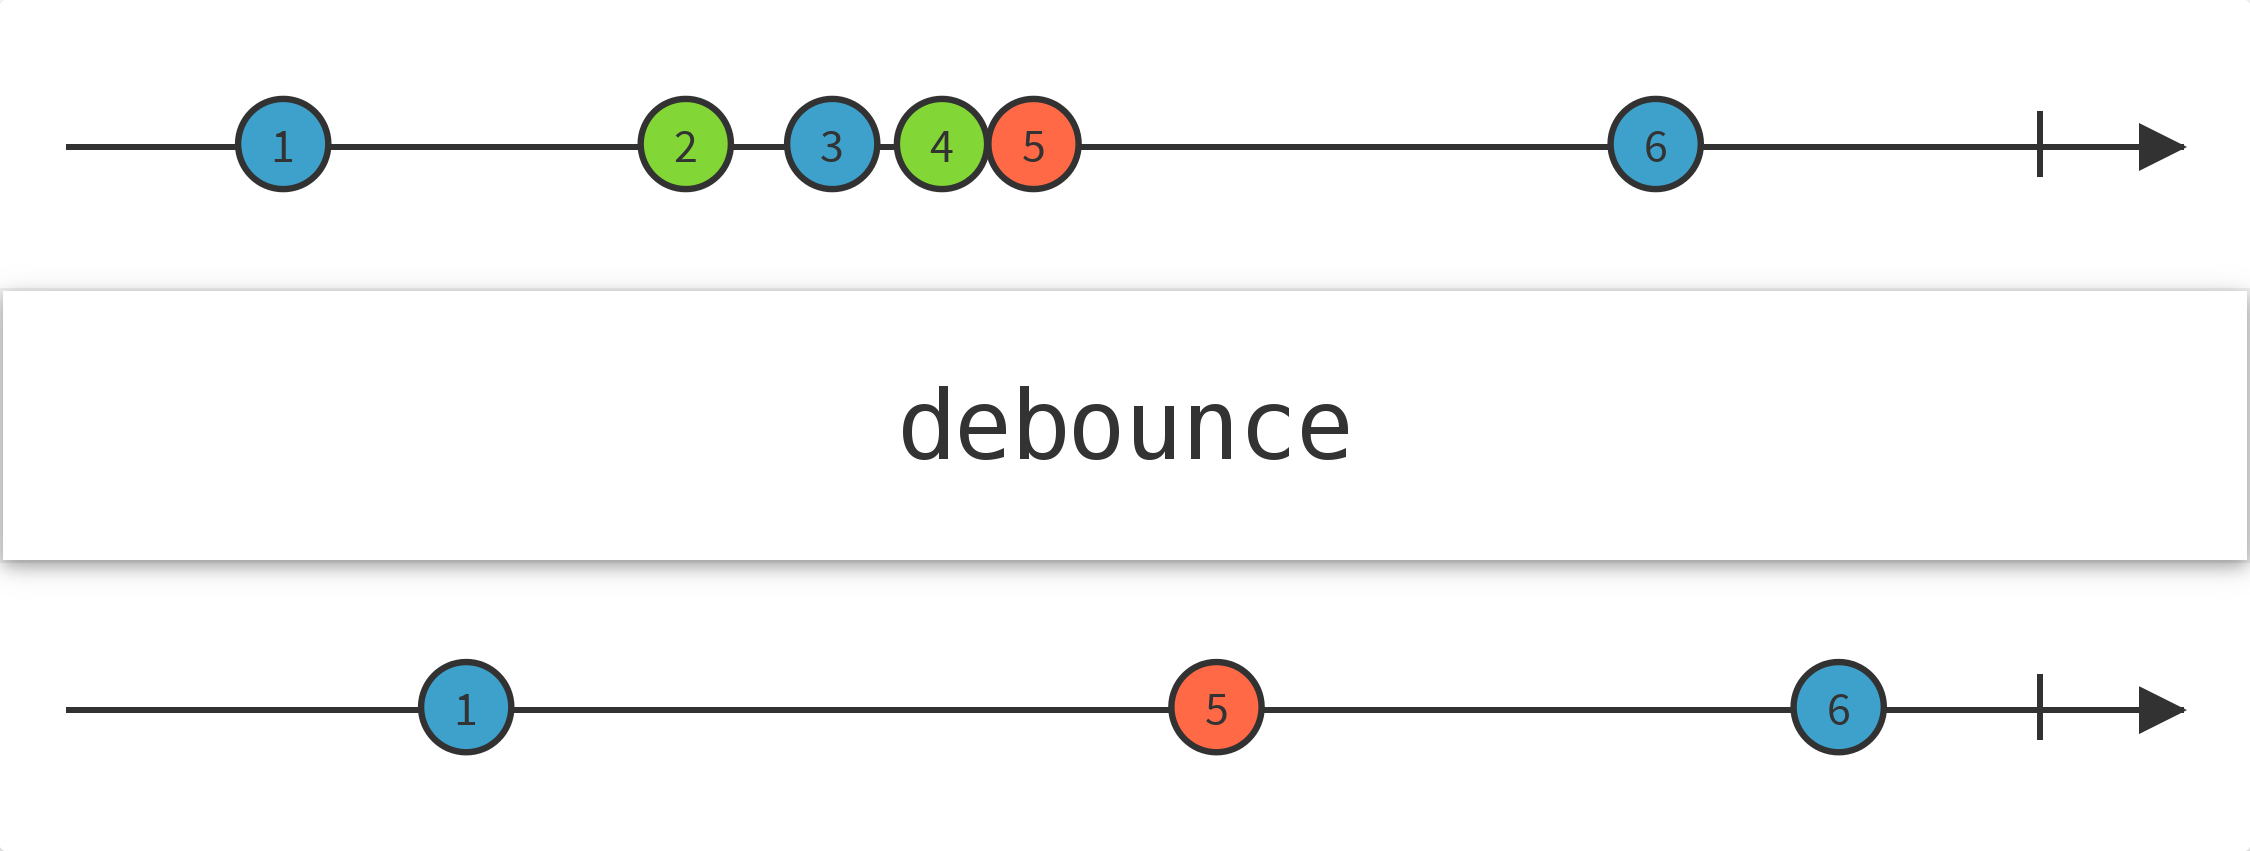
\includegraphics[width=0.8\textwidth]{images/reactivex-debounce}
  \caption{Der ReactiveX-Filter \texttt{debounce}}
  \label{fig:reactivex-debounce}
\end{figure}

Manchmal kann es auch notwendig sein, die eingehenden Werte zu transformieren. \idename{} macht von dieser Möglichkeit ausgiebig Gebrauch, um die Ergebnisse von \texttt{HTTP}-Operationen aus einer \texttt{JSON}-Darstellung in die interne Repräsentation zu wandeln. An dieser Stelle kann dann die aus der funktionalen Programmierung bekannte \texttt{map}-Funktion eingesetzt werden (Abbildung~\ref{fig:reactivex-map}).

\begin{figure}[h]
  \centering \includegraphics[width=0.8\textwidth]{images/reactivex-map}
  \caption{Der ReactiveX-Transformator \texttt{map}}
  \label{fig:reactivex-map}
\end{figure}

Die wesentliche Stärker dieser (und natürlich auch vieler weiterer) Operationen liegt vor allem in ihrer Kombinierbarkeit. So ist es mit den beiden vorgestellten Operatoren ein leichtes, die Veränderungen einer Abfrage leicht zeitlich verzögert (\texttt{debounce}) in einer textuellen Repräsentation (\texttt{map} mit \texttt{toSqlString}) auf der Oberfläche anzuzeigen. Der \idename{}-Kern nutzt daher die ReactiveX-Erweiterungen in Form der Javascript-Bibliothek "`RxJS"'\footnote{\url{https://github.com/Reactive-Extensions/RxJS}}.

\subsubsection{Existierende Implementierungen von Drag \& Drop-Editoren}

Die Drag \& Drop-Editoren sind allesamt von Grund auf vorgenommene Eigenentwicklungen, welche direkt auf der \texttt{HTML5}-Spezifikation aufsetzen. Im Rahmen des schon vorgestellten App Inventor (\fullref{sec:related-app-inventor}) wurde von Google allerdings ebenfalls eine quelloffene Bibliothek für Drag \& Drop-Editoren namens "`Blockly"' entwickelt\footnote{\url{https://developers.google.com/blockly/}}. Warum wurde für \idename{} also eine Eigenentwicklung forciert?

Um Blockly zu evaluieren ist ein sehr kleiner Prototyp zur Bearbeitung von \texttt{SQL}-Abfragen entwickelt worden (Abbildung~\ref{fig:blockly-eval-sql}). Dabei hat sich kein schlagender Grund gegen Blockly gefunden, stattdesen aber eine recht lange Liste von technischen und inhaltlichen Aspekten, die nicht so recht zu \idename{} passen:

\begin{itemize}[noitemsep]
\item Es handelt sich bei Blockly um eine Bibliothek für imperative Programmiersprachen, inklusive Code-Generatoren für zum Beispiel Python, Javascript, Lua, ... Eine Unterstützung von \texttt{HTML} oder \texttt{SQL} ist nicht vorgesehen und müsste selber implementiert werden.
  
\item Code-Elemente werden in Blockly standardmäßig frei auf einer zweidimensionalen Zeichenfläche platziert. Um innerhalb eines Kontextes auf Ereignisse zu reagieren ist dieser Ansatz sinnvoll. Für \idename{} gilt jedoch, dass jedes zu bearbeitende Element feste Einstiegspunkte hat: \texttt{SELECT} und \texttt{FROM} bei lesenden \texttt{SQL}-Abfragen, \texttt{<body>} und möglicherweise \texttt{<head>} für Webseiten. Die mehrfache Verwendung dieser Wurzelelemente ist inhaltlich nicht sinnvoll, eine freie Platzierung bietet keinen signifikanten Mehrwert.

\item Das von Blockly verwendete Datenmodell enthält Details zur grafischen Darstellung und eignet sich nicht gut zur abstrakten Repräsentation von \texttt{HTML} oder \texttt{SQL}. Dieses Format kommt daher im Hinblick auf andere Arten von Editoren, zum Beispiel einem \texttt{WYSIWYG}-Editor für Oberflächen, nicht als exklusives Format in Frage. Dementsprechend müsste immer zwischen den eigentlichen \idename{}-Formaten und Blockly hin- und zurück-übersetzt werden.
  
\item Blockly versteht sich nicht nur als Oberflächenbibliothek, sondern auch als Code-Generator. Dieser Aspekt wird in \idename{} aber losgelöst von der grafischen Repräsentationen durch einzelne Editoren betrachtet. Diese Funktionalität von Blockly müsste daher aktiv ignoriert werden, da einzelne Schnittstellen das Vorhandensein entsprechender Funktionalität voraussetzen.
  
\item Blockly geht zunächst von einem statisch großen Zeichenbereich aus. Um diesen in der Größe zu verändern, muss auf globale \texttt{onResize}-Ereignisse reagiert werden. \idename{} kommt hingegen mit ausschließlich per \texttt{CSS} gehandhabten Größenangeben aus, was im Endeffekt permanent korrekte Größenverhältnisse garantiert. Die offizielle "`Resizeable Blockly"'-Demo\footnote{\url{https://blockly-demo.appspot.com/static/demos/resizable/overlay.html}} lässt sich hingegen durch Nutzung der Entwicklerfunktionen zur Bildschirmgrößen-Vorschau in Chrome und Firefox aus dem Tritt bringen.
\end{itemize}

\begin{figure}[t]
  \centering \includegraphics[width=0.6\textwidth]{images/blockly/first-steps}
  \caption{Grundzüge eines \texttt{SQL}-Editors mit Blockly}
  \label{fig:blockly-eval-sql}
\end{figure}

Da \idename{} zumindest perspektivisch die Verwendung von unterschiedlichen Editoren für identische Inhalte vorsieht, ist Blockly damit keinesfalls endgültig aus der Welt. Spätestens bei einer hypothetischen Einbindung von "`echten"' Programmiersprachen in \idename{} wird eine Integration wieder zur Diskussion stehen.

\subsection{Server}

Der Server beschränkt sich auf drei wesentliche Aufgaben und ist dementsprechend von überschaubarem Umfang:

\begin{enumerate}[noitemsep]
\item Bereitstellung der statischen \texttt{HTML}- und (aus Typescript kompilierten) Javascript-Dateien, sofern kein "`normaler"' Webserver vorgeschaltet wird.
\item Entgegennehmen von Speicheranfragen und Prüfung auf deren Plausibilität beziehungsweise Befugnis.
\item Rendern der Webseiten für Endbenutzer.
\end{enumerate}

Die ersten beiden dieser Punkte werden unmittelbar von Sinatra unterstützt. Die Bereitstellung von statischen Daten funktioniert über die \texttt{send\_file(path)}-Methode, Authentifizierungen können über einen entsprechenden \texttt{HTTP}-Auth-Header angefordert werden. Um die eingehenden Daten zu validieren, werden alle Anfragen gegen ein \texttt{JSON}-Schema validiert. Das Rendern der Seiten für Endbenutzer ist hingegen etwas komplizierter, die Rahmenbedingungen dafür werden daher in diesem Kapitel etwas ausführlicher betrachtet.

\subsubsection{Nutzung von Subdomains}

\idename{}-Projekte werden unter jeweils eigenen Subdomains zur Verfügung gestellt. Das erhöht zwar die Anforderungen an die technische Infrastruktur, geht jedoch mit einer Reihe von Vorteilen einher. Die online bereitgestellte Fassung des Protoypen geht in Bezug auf die zur Verfügung stehenden Subdomains noch einen Schritt weiter: Die Domain für die Entwicklungsumgebung (\href{http://blattwerkzeug.de}{\texttt{blattwerkzeug.de}}) unterscheidet sich von jener für die Projekte (zum Beispiel \href{http://cyoa.blattzeug.de}{\texttt{cyoa.blattzeug.de}}).

Der hauptsächliche Grund für dieses Vorgehen ist die im Internet weitestgehend gültige Annahme, dass auf jeder (Sub-)Domain nur ein logischer Internetauftritt hinterlegt ist. Dass sich hinter einer \texttt{URL} wie \texttt{blatt\-werk\-zeug.de\-/project\-/pokemongo} eine völlig andere Seite als hinter \texttt{blatt\-werk\-zeug.de\-/project\-/cyoa} verbirgt, ist zwar in keinster Weise verboten, aber zumindest ungewöhnlich.

Praktisch werden Subdomains von vielen Suchmaschinen, sonstigen Angeboten im Internet und auch innerhalb der technischen Standards anders behandelt, als wenn die gleichen Inhalte als untergeordnete \texttt{URL} einer anderen Seite existierten. Das beginnt schon bei entscheidenden technischen Details: So können zum Beispiel Zertifikate für \texttt{SSL}-Verbindungen nur für Domains, nicht aber für Teile einer \texttt{URL} ausgestellt werden. Und Webseiten werden im Falle von unerwünschten Inhalten, zum Beispiel Phishing-Angriffen, üblicherweise auf Basis von Domainnamen gesperrt.

Darüber hinaus kann unter dieser Voraussetzung jede Webseite davon ausgehen, dass die gesamte Routing-Hierarchie nur ihr gehört. Die Subdomains erlauben also die Nutzung von absoluten Pfadangaben. Insbesondere um Bilder, \texttt{CSS}-Dateien oder JavaScript-Bibliotheken zu verlinken, ist das eine hilfreiche Garantie, welche viele unpraktische Probleme vermeidet.

\subsubsection{Rendervorgang}

Der wesentliche Inhalt des Rendervorgangs besteht im Sammeln der für die Anzeige notwendigen Daten, wie sie in Kapitel \fullref{sec:page-data-sources} beschrieben worden sind. Ein Großteil dieser Daten kann unmittelbar aus dem Datenmodell heraus\-gelesen werden: Die Ruby-Klassen für Projekte und Seiten verfügen über dezidierte Methoden zur Bereitstellung der Daten ihres Namensraumes (Listing~\ref{lst:server-project-render-data}). Die \texttt{GET}-Daten werden unmittelbar von dem serverseitigen Framework zur Verfügung gestellt.

\begin{lstlisting}[float=h, language=Ruby, caption={Bereitstellung der Renderdaten in der Projektklasse}, label={lst:server-project-render-data}]
# Retrieves the "site" hash that may be used during rendering.
#
# @return [Hash] Rendering-relevant data for a project
def render_params
  return {
    'name' => self.whole_description['name'],
    'id' => self.id,
    'description' => self.whole_description['description'],
  }
end
\end{lstlisting}

Um die Abfragen in das richtige Format zu bringen, ist hingegen ein wenig Aufwand erforderlich: Jede in einer Seite referenzierte Abfrage muss ausgeführt werden. Dieser Prozess erfolgt in zwei Schritten.

Zunächst werden die verfügbaren Parameter auf die tatsächlich benötigten Parameter abgebildet. Zur Erinnerung sei daher an dieser Stelle noch einmal die grundsätzliche Problematik erwähnt: Die Daten für die Seiten liegen in Namensräumen vor, die Parameter einer Abfrage wissen hingegen nichts von diesen Namensräumen. Listing~\ref{lst:server-project-query-prepare-params} zeigt, wie die einzelnen Mapping-Einträge einer referenzierten Abfrage in Namensraum und Schlüssel aufgespalten und dann unter dem in der Abfrage definierten Parameternamen verfügbar gemacht werden.

\begin{lstlisting}[float=p, language=Ruby, caption={Renderdaten einer Abfrage (1): Parameter binden}, label={lst:server-project-query-prepare-params}]
# Each query gets its own fresh set of parameters
params = {}

# Not-quite-so-wellformed models may omit the mapping, this
# shouldn't crash anything immediatly.
query_ref.fetch('mapping', {}).each do |mapping|
  # Extract all relevant indizes
  prov_prefix, prov_name = mapping.fetch('providingName').split "."
  parameter_name = mapping.fetch('parameterName')
  
  # And do the actual mapping
  mapped_value = initial_params
                 .fetch(prov_prefix)
                 .fetch(prov_name)
  params[parameter_name] = mapped_value
end
\end{lstlisting}

Nachdem die Parameter dann übersetzt worden sind, erfolgt die eigentliche Ausführung der Abfrage (Listing~\ref{lst:server-project-query-map-results}). Dabei werden die als \texttt{string[][]}-Array zurückgelieferten Rohdaten in ein Array von Hash-Maps übersetzt (\texttt{Dict<string, string>[]}). Nach dieser Präparation der Parameter und der Transformation der erhaltenen Zeilen kann das Ergebnis der Abfrage dann in die Renderdaten eingepflegt werden.

\begin{lstlisting}[float=p, language=Ruby, caption={Renderdaten einer Abfrage (2): Ausführen und transformieren}, label={lst:server-project-query-map-results}]
# Grab the actual query and execute it with the constructed parameters
query = @project.query_by_id(query_ref['queryId'])
result = @project.execute_sql(query.sql, params)

# Templating engines works much better with 'sensible' keys as names,
# so we map the column names into each row. This basically transforms
# rows like [1,2,3] to { "column-name-1" => 1, ... }
mapped = result['rows'].map { |r| Hash[result['columns'].zip r] }

# Rows with a single value allow a short-hand notation. The user
# shouldn't be forced to write {{ row[0].column }} every time he
# **knows** there is only a single row.
if query.single_row?
  if mapped.length == 1
    mapped = mapped.first
  else
    err_msg = "Got #{mapped.length} rows, expected exactly 1"
    raise DatabaseQueryError.new(@project, query.sql, params, err_msg)
  end
end

return (mapped);
\end{lstlisting}

Der eigentliche Rendervorgang wird von der Liquid-Bibliothek durchgeführt. Deren Interface ist aber wie in Kapitel \fullref{sec:eval-templating-language} beschrieben denkbar einfach: Übergeben wird ein String mit dem zu rendernden Template und die in diesem Kapitel beschriebene \texttt{HashMap} mit den zur Verfügung stehenden Daten.

\subsection{Unerwartete Hindernisse}
\label{sec:unexpected-problems}

Im Laufe der \idename{}-Entwicklung traten, vornehmlich bei der Entwicklung des Webclients, einige unerwartete Hindernisse auf. Jene Probleme, die subjektiv betrachtet wesentlich mehr Zeit gekostet haben als eingeplant war, werden an dieser Stelle kurz erwähnt.

\subsubsection{Instabile API von Angular 2}

Zum Start der Entwicklung von \idename{} befand sich Angular 2 gerade in der Version \texttt{2.0.0-beta.0}. Auf diese initiale Version folgten 17 weitere Beta-Veröffentlichungen und 7 "`Release-Candidates"'. Alle in diesen Veröffentlichungen getätigten "`Breaking Changes"' mussten von \idename{} mitgemacht und nachvollzogen werden. Zu den besonders schwerwiegenden Umbauten gehören dabei die folgenden Anlässe:

\begin{itemize}[noitemsep]
\item Das interne Routing-Modell wurde zweimal komplett umgeschrieben, dabei waren jedes Mal manuelle Änderungen an den Routendefinitionen nötig\footnote{Siehe \url{http://stackoverflow.com/questions/38039294/} und \\ \url{http://stackoverflow.com/questions/38879529/\#38952908}}. Zum aktuellen Zeitpunkt liegt der Router daher schon in Version 3 vor, während Angular 2 noch auf Version 2 verweilt.
\item Die interne Darstellung von Abhängigkeiten einzelner Komponenten wurde mit dem Release-Kandidaten 5 komplett überarbeitet. Bisher hatten Komponenten Abhängigkeiten selber referenziert, nun sollen diese dafür in ein neu entwickeltes Modulsystem einsortiert werden.
\item Die Syntax der Templatingsprache wurde in Bezug auf die Angabe von Referenzen verändert. Dabei wurden Schlüsselwörter verändert und gestrichen, was eine komplette Durchsicht aller Template-Dateien erforderte.
\end{itemize}

\subsubsection{Fehlerhafte Codegenerierung des Typescript-Compilers}

Der verwendete Typescript-Compiler hat zum Zeitpunkt der Anfertigung dieser Arbeit einen bekannten Bug in der Codegenerierung\footnote{\url{https://github.com/Microsoft/TypeScript/issues/4341}}, um den wiederholt herumgearbeitet werden musste. Konkret äußert sich dieser Fehler, wenn die Definition der Oberklasse einer sich davon ableitenden Klasse erst im Nachhinein erfolgt (Listing \ref{lst:ts:class-order-bug}). In diesem Fall kommt es zu keiner Warnung durch den Compiler, sondern zu einem Laufzeitfehler im kompilierten Javascript-Code. Das Beispiel ist an dieser Stelle natürlich besonders plakativ, der Fehler tritt aber in identischer Art und Weise bei komplexen Hierarchien aus \texttt{import}-Anweisungen auf.

\lstinputlisting[float=p, language=JavaScript, caption=Falsche Reihenfolge der Klassendefinition, label=lst:ts:class-order-bug]{snippets/class-inheritance-order-bug.ts}

\subsubsection{Verworfene Implementierung eines reinen WYSIWYG-Seiten-Editors}

Vor dem im aktuellen Prototypen verwendeten Block-Editor (zu sehen auf zum Beispiel Abbildung~\ref{fig:screen-ui-editor-block} oder im Anhang \fullref{sec:project-examples}) wurde noch ein reiner WYSIWYG-Editor entwickelt. Dieser ist in der Lage, beliebige Layouts aus Zeilen und Spalten mit einer akkuraten Vorschau zu versehen. Der nächste Schritt in der Implementierung wäre neben der Vorschau von Knöpfen und Eingabefeldern die Darstellung der Datentabellen gewesen (Abbildung~\ref{fig:discarded-wysiwyg-page-editor}).

Die Weiterentwicklung wurde dann jedoch nach einem Gespräch mit Dr. Frank Huch in einer gemeinsamen Entscheidung gestoppt: Dieser Editor wäre eine weitere Insellösung gewesen, mit der die Lernenden zwar hätten schnell erste Erfolge vorweisen können, dabei die technischen Hintergründe jedoch nicht verstanden hätten. So weit sollte die "`Motivation durch praktisch vorzeigbare Ergebnisse"' dann doch nicht getrieben werden, schließlich handelt es sich bei \idename{} in erster Linie immer noch um ein Lehrprogramm. Vollständig Vergebens waren die investierte Zeit dennoch nicht: Das entwickelte Datenmodell für die Seiten konnte beibehalten werden, der serverseitige Code zum Rendern ebenfalls.

\begin{figure}[p]
  \centering \includegraphics[width=\textwidth]{images/screenshots/20160731/esqulino-editor-page-keyboard-input-partial}
  \caption{Entwickleransicht des verworfenen WYSIWYG-Seiten-Editors}
  \label{fig:discarded-wysiwyg-page-editor}
\end{figure}

%%% Local Variables:
%%% mode: latex
%%% TeX-master: "thesis"
%%% End:
